\let\negmedspace\undefined
\let\negthickspace\undefined
\documentclass[journal]{IEEEtran}
\usepackage[a5paper, margin=10mm, onecolumn]{geometry}
%\usepackage{lmodern} % Ensure lmodern is loaded for pdflatex
\usepackage{tfrupee} % Include tfrupee package

\setlength{\headheight}{1cm} % Set the height of the header box
\setlength{\headsep}{0mm}     % Set the distance between the header box and the top of the text

\usepackage{gvv-book}
\usepackage{gvv}
\usepackage{cite}
\usepackage{amsmath,amssymb,amsfonts,amsthm}
\usepackage{algorithmic}
\usepackage{graphicx}
\usepackage{textcomp}
\usepackage{xcolor}
\usepackage{txfonts}
\usepackage{listings}
\usepackage{enumitem}
\usepackage{mathtools}
\usepackage{gensymb}
\usepackage{comment}
\usepackage[breaklinks=true]{hyperref}
\usepackage{tkz-euclide} 
\usepackage{listings}
% \usepackage{gvv}                                        
\def\inputGnumericTable{}                                 
\usepackage[latin1]{inputenc}                                
\usepackage{color}                                            
\usepackage{array}                                            
\usepackage{longtable}                                       
\usepackage{calc}                                             
\usepackage{multirow}                                         
\usepackage{hhline}                                           
\usepackage{ifthen}                                           
\usepackage{lscape}
\begin{document}

\bibliographystyle{IEEEtran}
\vspace{3cm}
\title{12.8.3.18}
\author{EE24BTECH11025 - GEEDI HARSHA}
% \maketitle
% \newpage
{\let\newpage\relax\maketitle}

\renewcommand{\thefigure}{\theenumi}
\renewcommand{\thetable}{\theenumi}
\setlength{\intextsep}{10pt} % Space between text and floats


\numberwithin{equation}{enumi}
\numberwithin{figure}{enumi}
\renewcommand{\thetable}{\theenumi}

\textbf{Question:}
The area of the circle \(x^2 + y^2 = 16\) exterior to the parabola \(y^2 = 6x\) is:


\solution

The circle is given by:
\begin{align*}
x^2 + y^2 &= 16 \quad \Rightarrow \quad r = 4
\end{align*}

The parabola is given by:
\begin{align*}
y^2 &= 6x
\end{align*}
\subsection*{Intersection Points}
Equating \(x^2 + y^2 = 16\) and \(y^2 = 6x\), we substitute \(y^2 = 6x\) into the circle equation:
\begin{align*}
x^2 + 6x &= 16 \quad \Rightarrow \quad x^2 + 6x - 16 = 0
\end{align*}

Solving the quadratic equation:
\begin{align*}
x &= \frac{-6 \pm \sqrt{6^2 - 4(1)(-16)}}{2(1)} = \frac{-6 \pm \sqrt{100}}{2} = \frac{-6 \pm 10}{2} \\
x &= 2 \quad \text{and} \quad x = -8
\end{align*}

Thus, the intersection points are \((2, \pm \sqrt{12})\).

\subsection*{Area Calculation}
The area outside the parabola and inside the circle is given by:
\begin{align*}
\text{Area} &= \text{Total Circle Area} - 2 \times \int_0^2 \sqrt{6x} \, dx
\end{align*}

1. Total circle area:
\begin{align*}
A_{\text{circle}} &= \pi r^2 = 16\pi
\end{align*}

2. Area under the parabola:
\begin{align*}
\int_0^2 \sqrt{6x} \, dx &= \int_0^2 \sqrt{6} \sqrt{x} \, dx = \sqrt{6} \int_0^2 x^{1/2} \, dx \\
&= \sqrt{6} \left[\frac{2}{3}x^{3/2}\right]_0^2 \\
&= \sqrt{6} \cdot \frac{2}{3} \cdot (2^{3/2}) = \frac{4\sqrt{6}}{3}
\end{align*}

Thus, the area outside the parabola is:
\begin{align*}
\text{Area} &= 16\pi - \frac{8\sqrt{6}}{3} \\
&= \quad \frac{4}{3}(4\pi - \sqrt{3})
\end{align*}




\textbf{Computational Solution}\\

The \textbf{Trapezoidal} rule for approximating the integral of a function \(f(x)\) from \(a\) to \(b\) is given by:

\begin{align*}
\int_a^b f(x) \, dx &\approx \frac{h}{2} \left[ f(a) + 2 \sum_{i=1}^{n-1} f(x_i) + f(b) \right]
\end{align*}
where \(h = \frac{b - a}{n}\) is the width of each subinterval\\
 \(x_i = a + ih\) for \(i = 1, 2, \dots, n-1\).\\

In this case, \(f(x) = \sqrt{6x}\), and we are integrating from \(x = 0\) to \(x = 2\).


We will use \(n = 4\) subintervals for this approximation. Therefore, the width of each subinterval is:

\begin{align*}
h &= \frac{2 - 0}{4} = 0.5
\end{align*}

The points \(x_i\) are:

\begin{align*}
x_0 &= 0, \quad x_1 = 0.5, \quad x_2 = 1, \quad x_3 = 1.5, \quad x_4 = 2
\end{align*}

The corresponding function values are:

\begin{align*}
f(x_0) &= \sqrt{6(0)} = 0, \\
f(x_1) &= \sqrt{6(0.5)} = \sqrt{3}, \\
f(x_2) &= \sqrt{6(1)} = \sqrt{6}, \\
f(x_3) &= \sqrt{6(1.5)} = \sqrt{9} = 3, \\
f(x_4) &= \sqrt{6(2)} = \sqrt{12} = 2\sqrt{3}
\end{align*}

Now, we apply the trapezoidal rule:

\begin{align*}
\int_0^2 \sqrt{6x} \, dx &\approx \frac{0.5}{2} \left[ 0 + 2 \left( \sqrt{3} + \sqrt{6} + 3 \right) + 2\sqrt{3} \right] \\
&= 0.25 \left[ 0 + 2\sqrt{3} + 2\sqrt{6} + 6 + 2\sqrt{3} \right] \\
&= 0.25 \left[ 4\sqrt{3} + 2\sqrt{6} + 6 \right]
\end{align*}
\begin{figure}[h]
    \centering
    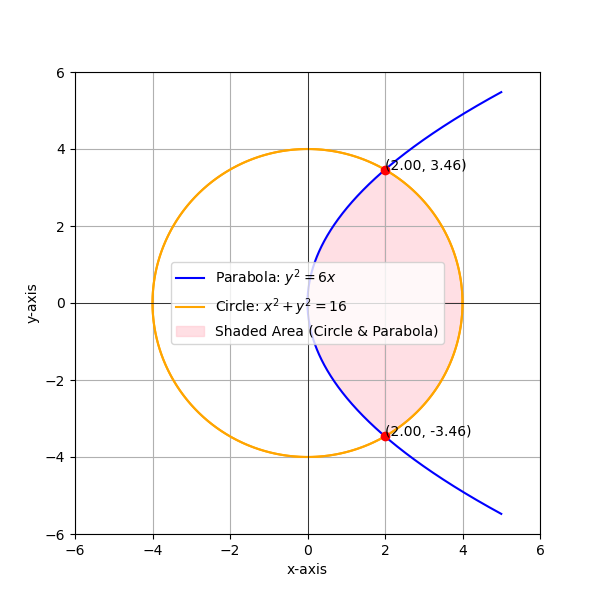
\includegraphics[width=\textwidth]{figs/fig.png}
\end{figure}
\end{document}

